\chapter{Atividade Econômica}
\par A eclosão da pandemia do coronavírus tem se mostrado o maior choque enfrentado pela economia brasileira, tanto pela demanda com a contração do consumo das famílias e dos investimentos, quanto pelo lado da oferta, com empresas indo à falência. Compondo a isso se tem a fragilidade fiscal do Estado brasileiro e a alta taxa de desemprego desde a recessão de 2015/2016. Dado este contexto, cria-se cenário preocupante para a economia brasileira como um todo.
\par Nesse sentido, espera-se também um grande choque na economia tocantinense. Os indicadores que serão apresentados ao longo das seções deste Boletim farão um retrato de como esse grande choque afetou e poderá afetar a economia do nosso estado.
\begin{smbox}[label={labelbox},nameref={Cálculo do PIB e as suas óticas}]{Cálculo do PIB e as suas óticas}
	O Produto Interno Bruto (PIB) é a soma de todos os bens e serviços finais produzidos por um país. É possível calcula-lo pela ótica da oferta, somando tudo aquilo que é produzido por todos os setores, pela ótica da demanda, somando o consumo das famílias, consumo do governo, investimentos e exportações liquidas (exportações menos importações) e também pela ótica da renda, somando toda renda da população. O resultado das três óticas é sempre o mesmo.
\end{smbox}
\begin{figure}[!h]
	\begin{subfigure}{\linewidth}
		\caption{Expectativa de crescimento anual do PIB}
		\subcap{Por setor}
		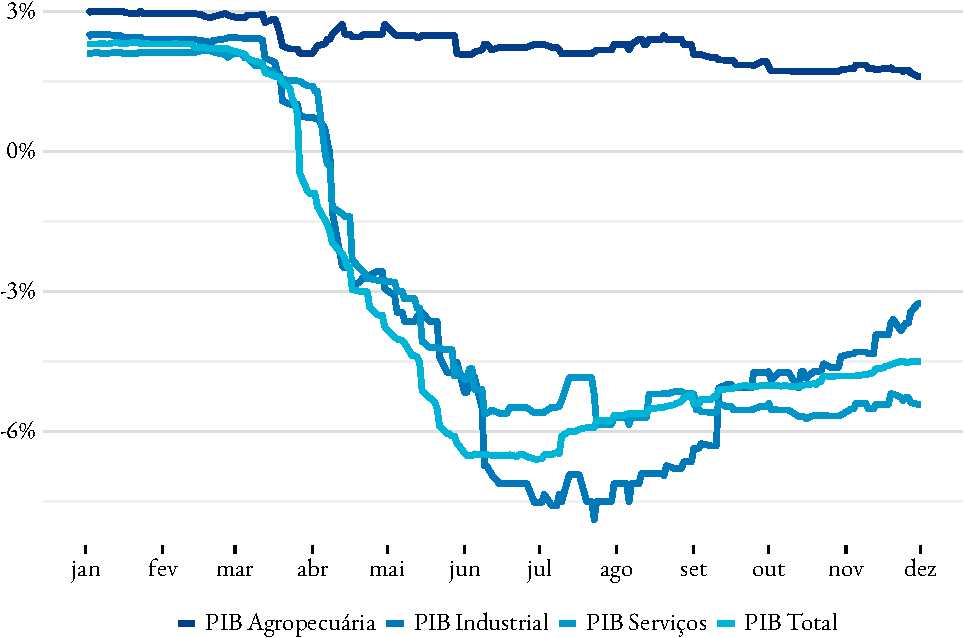
\includegraphics{fig/pib_expec-1.pdf}
		\source{Banco Central do Brasil/Relátorio Focus}
	\end{subfigure}
	\begin{subfigure}{\linewidth}
		\caption{Variação trimestral do PIB pelo lado da demanda}
		\subcap{Com ajuste sazonal}
		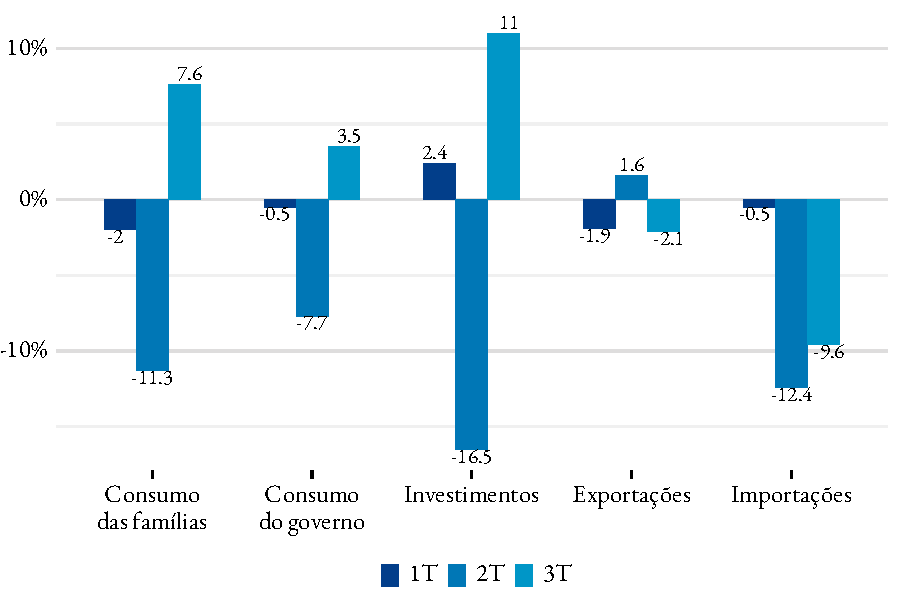
\includegraphics{fig/pib_demanda.pdf}
		\source{IBGE}
	\end{subfigure}
	\begin{subfigure}{\linewidth}
		\caption{Variação trimestral do PIB pelo lado da oferta}
		\subcap{Com ajuste sazonal}
		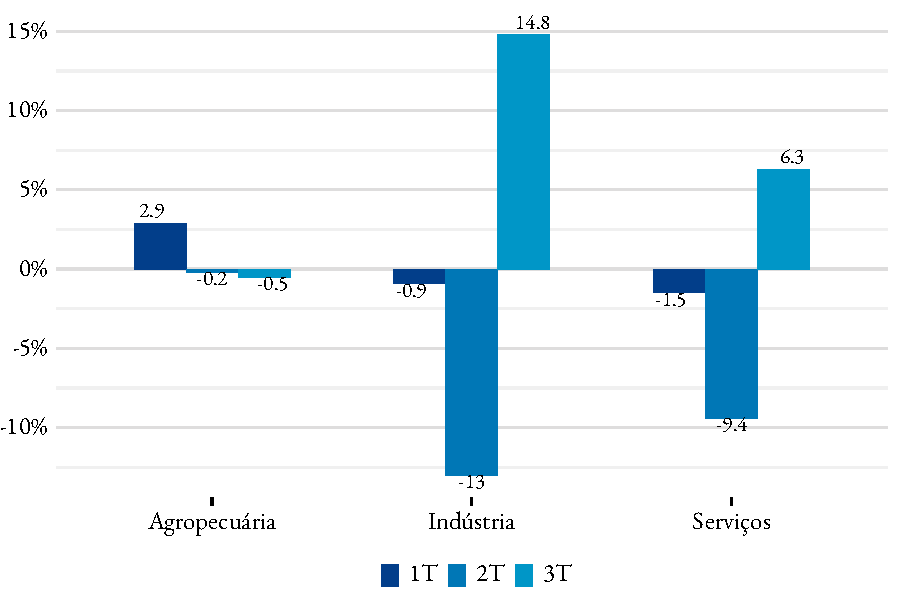
\includegraphics{fig/pib_oferta.pdf}
		\source{IBGE}
	\end{subfigure}
\end{figure}
\par Como pode ser visto na Figura 1.1, nos três primeiros trimestres de 2020 o PIB brasileiro encolheu 1,5\% e 9,6\%, nos dois primeiros trimestres e teve um crescimento de 7,7\%, que apesar de alto, ainda não foi suficiente para repor as perdas no início do ano. Esses resultados foram os primeiros sinais dos efeitos da pandemia da COVID-19, sendo que seu resultado negativo em partes explicados pelas medidas de fechamento de comércios e serviços a fim de evitar a propagação do vírus, sobretudo no segundo semestre.
\par Olhando o lado da demanda é possível ver uma queda generalizada sobre todos os componentes, com exceção das Exportações. Chama a atenção as fortes quedas no segundo trimestre, sobretudo no Consumo das famílias, Investimentos e Importações. No movimento de retomada do terceiro semestre é possível observar que grande parte do aumento de 7,7\% é explicado pela retomada do Consumo das famílias e Investimentos, tanto pelos bons resultados neste trimestre, mas também pelo tamanho desses componentes dentro da composição do PIB.
\par Pelo lado da oferta o único setor com resultados mais estáveis foi o Agropecuário, setor menos afetado pelas medidas de isolamento, e o que em parte explica o bom desempenho das exportações no lado da demanda. No setor de serviços, que representa nada menos do que 72\% do PIB, as quedas de 1.5\% e 9,4\% nos dois primeiros trimestres pesaram bastante. Já as quedas de 0,9\% e 13\% da indústria demonstram a fragilidade desse setor dentro da economia brasileira.
\par Nesse sentido, se coloca um grande desafio para economia tocantinense que é o de superar esse grande choque nunca antes visto na história do nosso jovem estado. Como já mencionado, é esperado que todas as variáveis discutidas ao longo deste Boletim sofram um forte impacto, tanto no curto, quanto no longo prazo. Pensar e discutir maneiras de lidar com esse choque adverso é um tema primordial na recuperação pós-pandemia para que a economia do nosso estado possa ter uma boa recuperação e para que se aumente a qualidade de vida do cidadão tocantinense ao longo de todo o estado.

\begin{figure}[!h]
	\begin{subfigure}{\linewidth}
		\caption{Atividade Econômica do Estado}
		\label{fig:pmc}
		\subcap{Variação acumulada no ano (base: igual período do ano anterior)}
		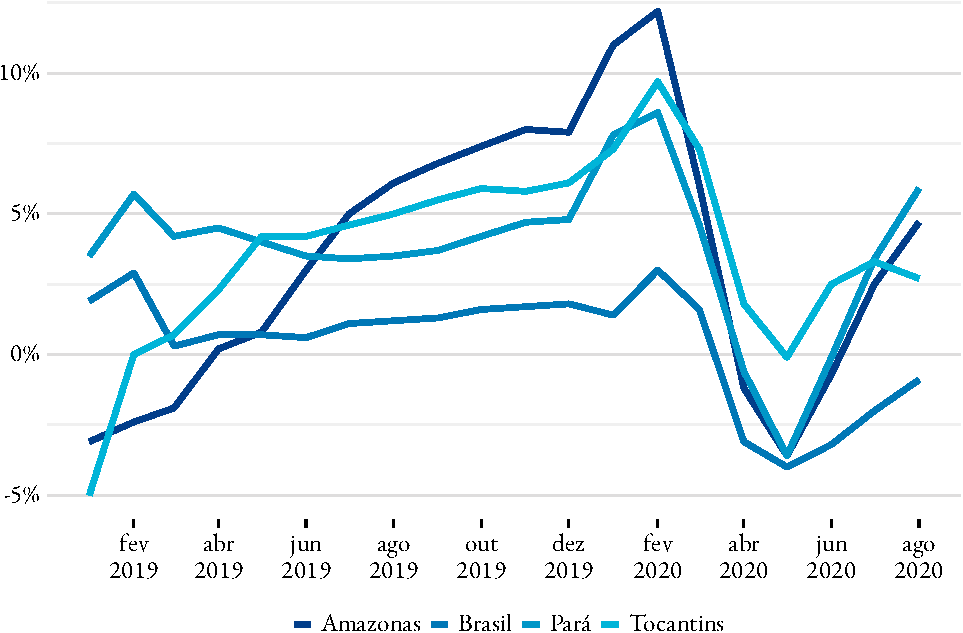
\includegraphics{fig/pmc_ibge-1.pdf}
		\source{IBGE}
	\end{subfigure}
\end{figure}
